\documentclass{article}

\title{EDA322 Digital Design -- Exam kit \\
  \small Revision: 1 (2018-06) -- Taube \& Jassob
  %% \normal Revision: X (date) -- Authors
}

\usepackage[includeheadfoot, top=1.0cm, bottom=2cm]{geometry}
\usepackage{hyperref, graphicx, parskip, lastpage}

\begin{document}
\maketitle
\tableofcontents

\newpage

\section{Introduction}
This is an exam kit for the course Digital Design given at Chalmers
University of Technology to second-year student on the Computer
Science and Engineering program.

The course is given by the Computer Engineering division at the
Computer Science and Engineering department.

The course is at the time of writing (2018) given in English and
therefore this exam kit is also written in English.

\subsection{Motivation}
Digital Design is a course that covers {\it a lot} and since there
usually are not very good answers to old exams it can be a difficult
course to retake if one does not attend every lecture.

This exam kit attempts to make it easier to study the course without
the aid of the lectures by including more thorough explanations and,
when needed, visualizing such explanations with step-by-step pictures.

\subsection{Structure}

This exam kit is divided into three sections:
\begin{itemize}
\item Introduction (which you are currently reading);
\item Theory \\
  contains a summary of the important parts of the course's theory
\item Quiz \\
  contains answers to quizzes given in lectures, good for quickly
  assessing what you might need to study more.
\end{itemize}

\newpage

\section{Theory}

\subsection{Configurable and non-configurable hardware}
There are different types of circuits and they come with their own set
of advantages and disadvantages. In this course we make the
distinction between reconfigurable hardware and non-reconfigurable
hardware. The two main types of circuits discussed in the course is
ASICs and FPGAs.

\subsubsection{ASIC (Application Specific Integrated Circuit)}
A non-reconfigurable circuit. The hardware of an ASIC can not be
changed after production. The static, specialized nature of this kind
of chips makes them energy-efficient and high-performing, but also
expensive to produce due to its high NRE\footnote{Non-recurring
  engineering, the one-time cost to research, design, develop and test
  a product} cost. Viable if many chips of the same kind and a
specific purpose is required (e.g. graphic card).

\subsubsection{FPGA (Field Programmable Gate Array)}
A specific type of reconfigurable circuit that contains a lot of
different circuit elements (for instance logic blocks, interconnects,
RAM memory blocks, multipliers etc) and is configurable by a
bitstream. This bitstream specifies how the circuit elements should
behave and the way they are connected to each other. Therefore, by
changing the configuration bitstream of an FPGA one can change the
functionality of it, or reconfigure it.

Compared to implementing circuit logic in ASICs, an FPGA design would
probably result in higher power consumption and often lower
performance, but since the chip is reconfigurable flaws in the design
can be fixed by updating the design and loading it to the FPGA,
resulting in a lower NRE cost (both in materials and time due to
quicker ``verify-and-fix'' iterations). A common use of FPGAs is
therefore to prototype a circuit design on an FPGA and then create
ASICs when the design is final.

FPGAs are also good choice if the volume of circuits is not big enough
to motivate the high cost of producing ASICs or if the flexibility of
reconfiguration is valuable (for instance to fix hardware bugs in a
system, or just re-use if a use case is not needed anymore).

For more information of FPGAs and their applications, we refer to the
wikipedia
\href{https://en.wikipedia.org/wiki/Field-programmable_gate_array#Applications}{article}
or section \ref{sec:rec-hw} which describes reconfigurable hardware in
more detail.

\subsection{Adders}

Adders are circuits that produce the sum of their input. The most
basic of adders are the Half Adder (abbreviation HA) which can be used
to add two 1-bit signals {\bf A} and {\bf B}. Implementation of a HA
is shown in figure \ref{fig:ha}. {\bf S} and {\bf C} are two 1-bit
output signals where {\bf S} is the 1-bit sum of {\bf A} and {\bf B}
and {\bf C} is the carry that tells us if the addition overflowed (i.e
{\bf A} and {\bf B} are both 1) or not.

\begin{figure}[ht]
  \centering
  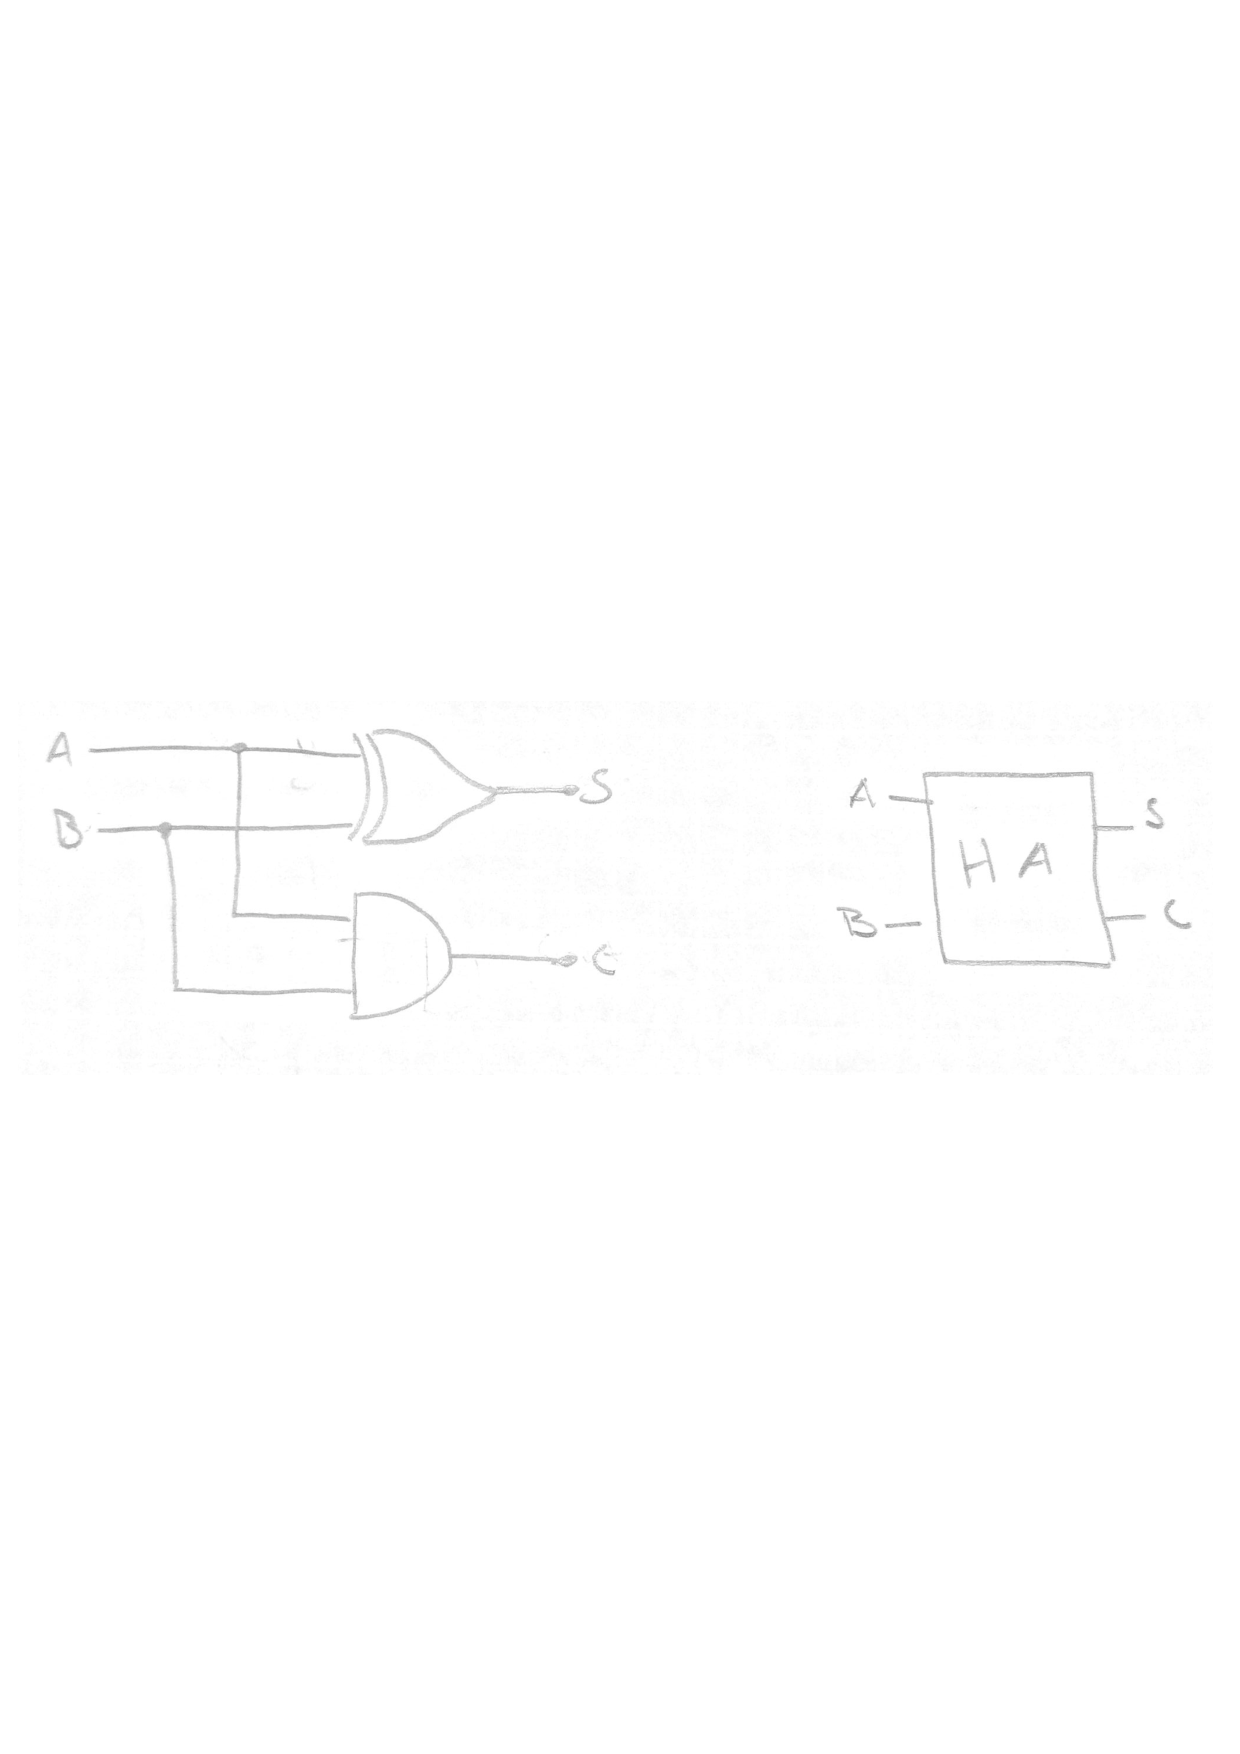
\includegraphics[width=10cm]{images/HA.pdf}
  \caption{Implementation of a 1 bit Half adder. Gate-level diagram to
    the left and a block diagram to the right. A and B are two 1-bit
    input signals and S and C are two 1-bit output signals. C is used
    to signal that an addition has overflowed, i.e if both A and B are
    1.}
  \label{fig:ha}
\end{figure}


If we want to add numbers represented by more bits than one we can
chain multiple 1-bit adders together. But how do we know if the last
addition overflowed or not? Simple, we'll just combine two half adders
where one takes care of the result of {\bf A} + {\bf B} and the other
takes care of the input carry (the overflow marker of last addition).
This arrangement of two half adder is called a Full Adder
(implementation is shown in figure \ref{fig:fa}) and still only sums
single-bit signals, but due to the ``carry in''-signal we can chain it
together to create multiple-bit adders.

\begin{figure}[ht]
  \centering
  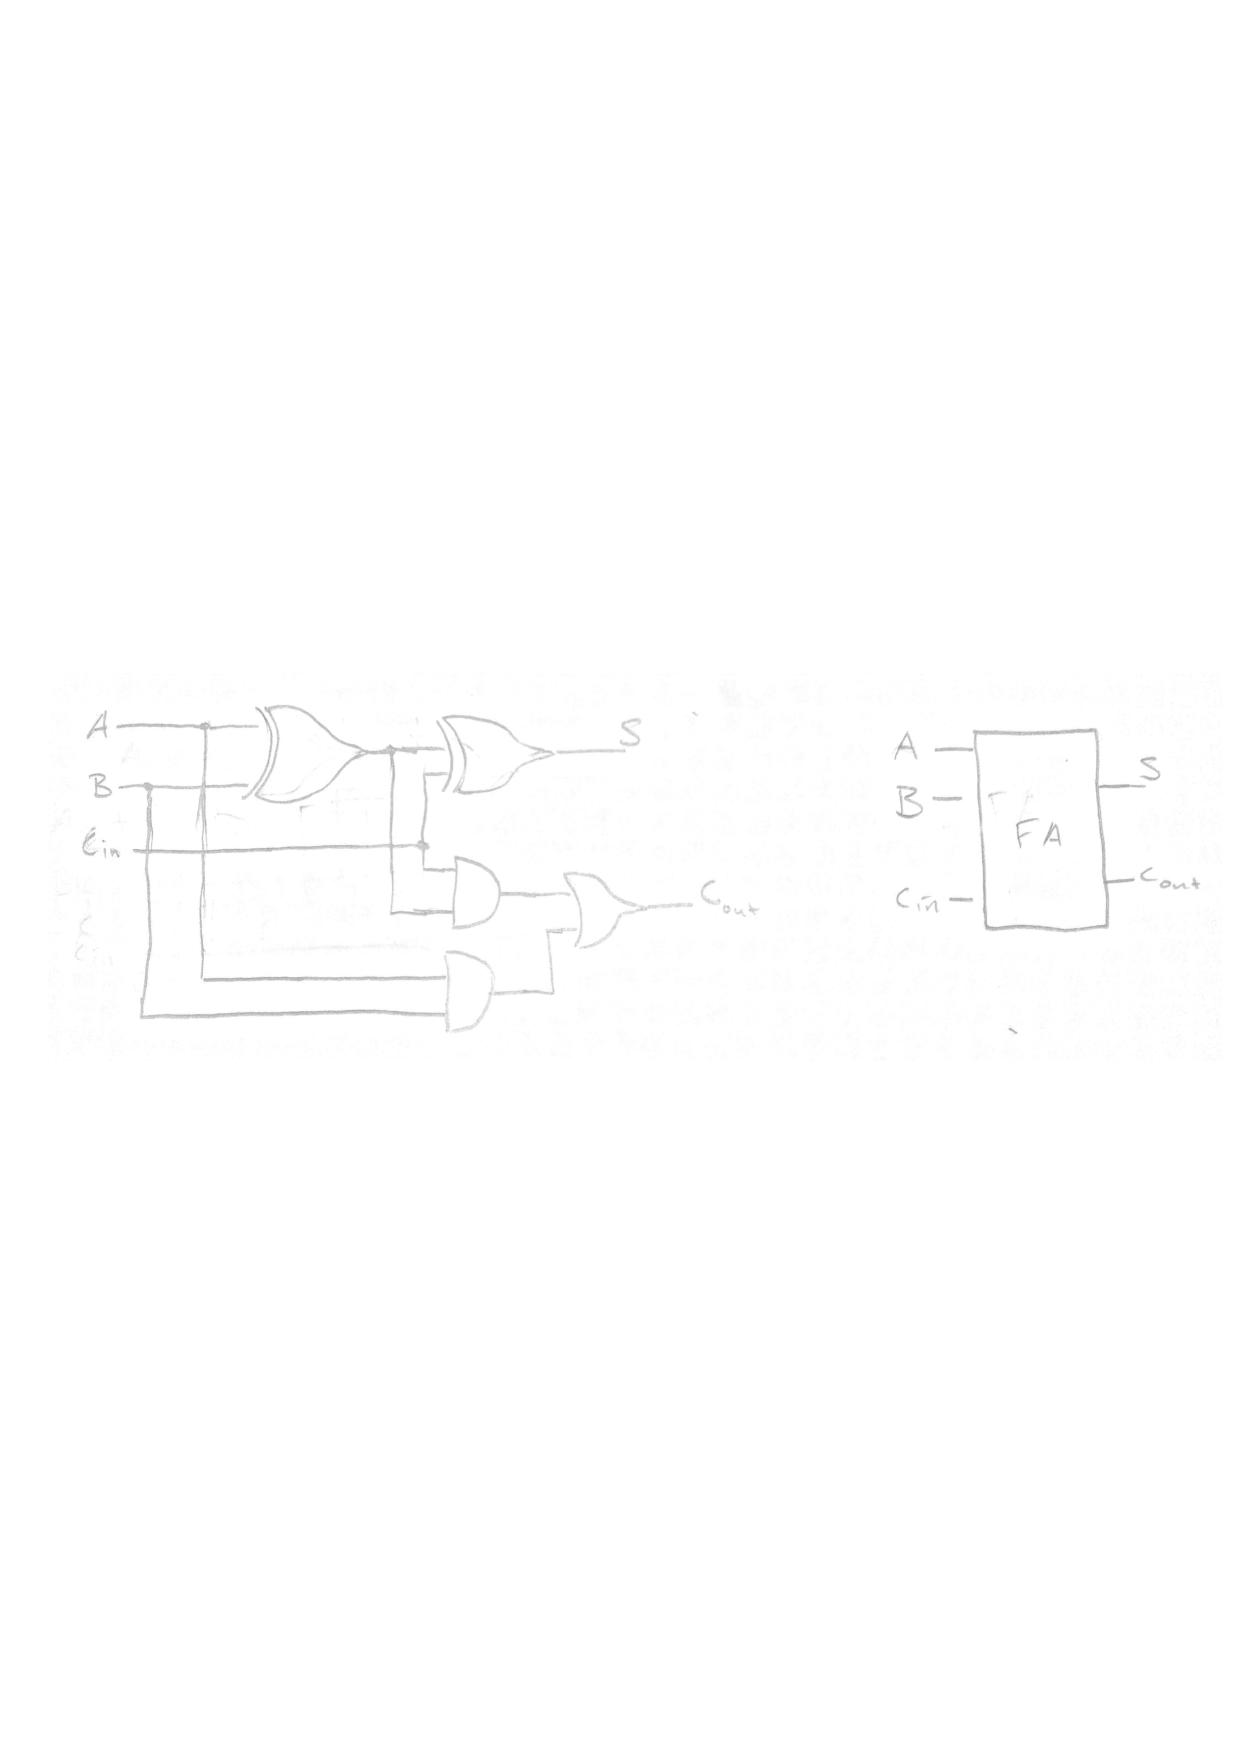
\includegraphics[width=10cm]{images/FA.pdf}
  \caption{Implementation of a 1 bit Full Adder. Gate-level diagram to the left and a block diagram to the right.}
  \label{fig:fa}
\end{figure}

Connecting two or more FAs by sending the carry out from the previous
FA to the carry in on the current FA is called a Ripple Carry Adder
(RCA) due to the way the carry ``ripples'' through the adders, from
the least significant adder to the most significant adder.

A simple 2-bit RCA is shown in figure \ref{fig:2fa}. The right-most
part of figure \ref{fig:2fa} is commonly used in block-levels as FAs
are common building blocks for building more complex adding circuits.

\begin{figure}[ht]
  \centering
  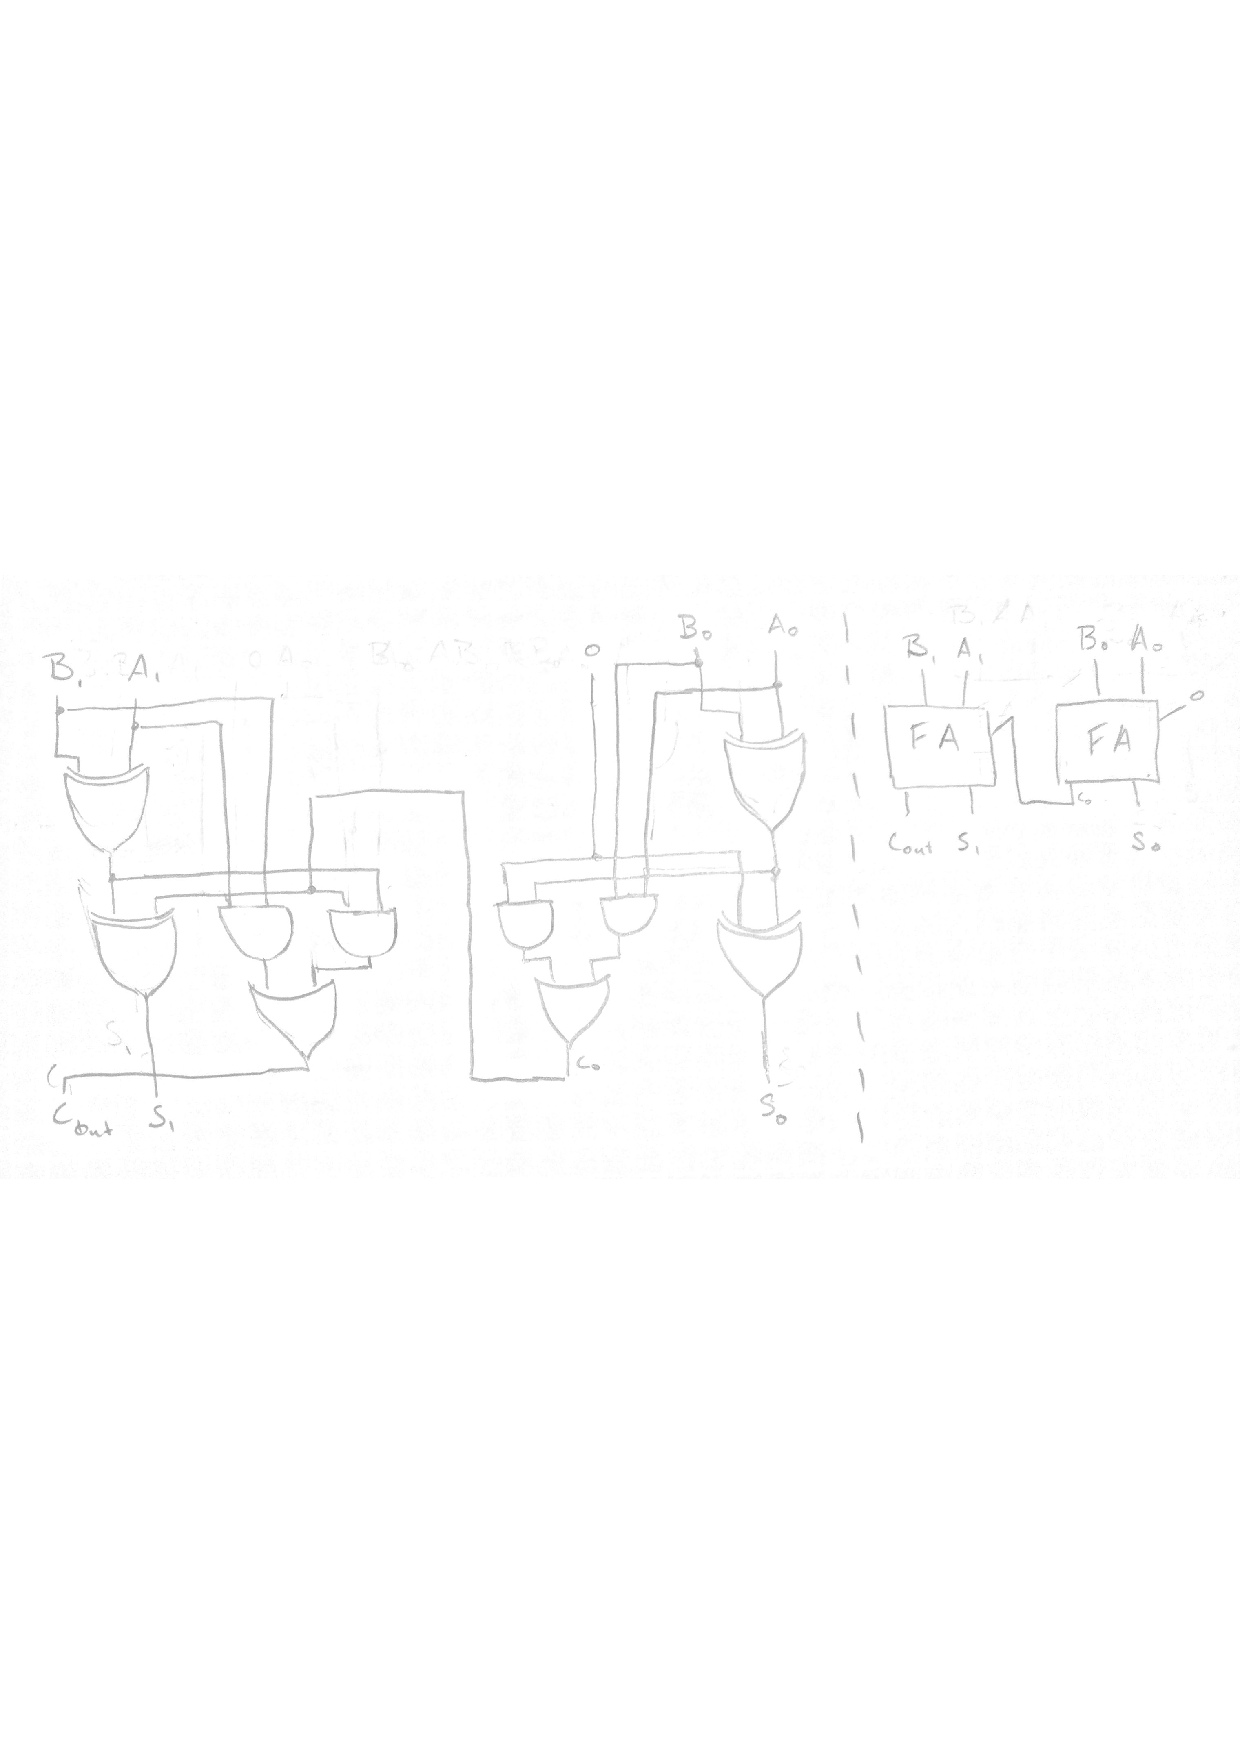
\includegraphics[width=10cm]{images/2b-FA.pdf}
  \caption{Implementation of a 2 bit Full Adder. Gate-level diagram to the left and a block diagram to the right.}
  \label{fig:2fa}
\end{figure}

Since every FA in an RCA depends on the carry out of the previous FA
no parallellisation is possible, the additions must be done in
sequence. This poses a linear time delay that depends on the number of
bits in the digits (or number of FAs). If we knew what the carry of
the previous addition will be we could in that case start start our
calculation before the previous calculation is completed {\it since
  the current calculation only depends on the last carry}. One simple
solution is to calculate two different versions of our sum, one where
the carry is 1 and one where the carry is 0 and then when the actual
carry is received we just select (with a MUX for instance) the correct
sum and carry from our calculation.

This is in fact the basis for the Carry-Select Adder (which is shown
in figure \ref{fig:4csa}). A CSA is basically an RCA where some FAs are
duplicated (they add the same input) but they are fed with a fixed
carry. This has the benefit that every FA that is fed a fixed carry
can start calculating at the same instance as the least significant FA
in the CSA and then the successor of these FAs with fixed carries can
continue doing their work. Essentially we've split up those parts in
the RCA into two identical parts that just differs in the initial
carry in. When the carry in arrives it selects which result the
circuit should output.

\begin{figure}[ht]
  \centering
  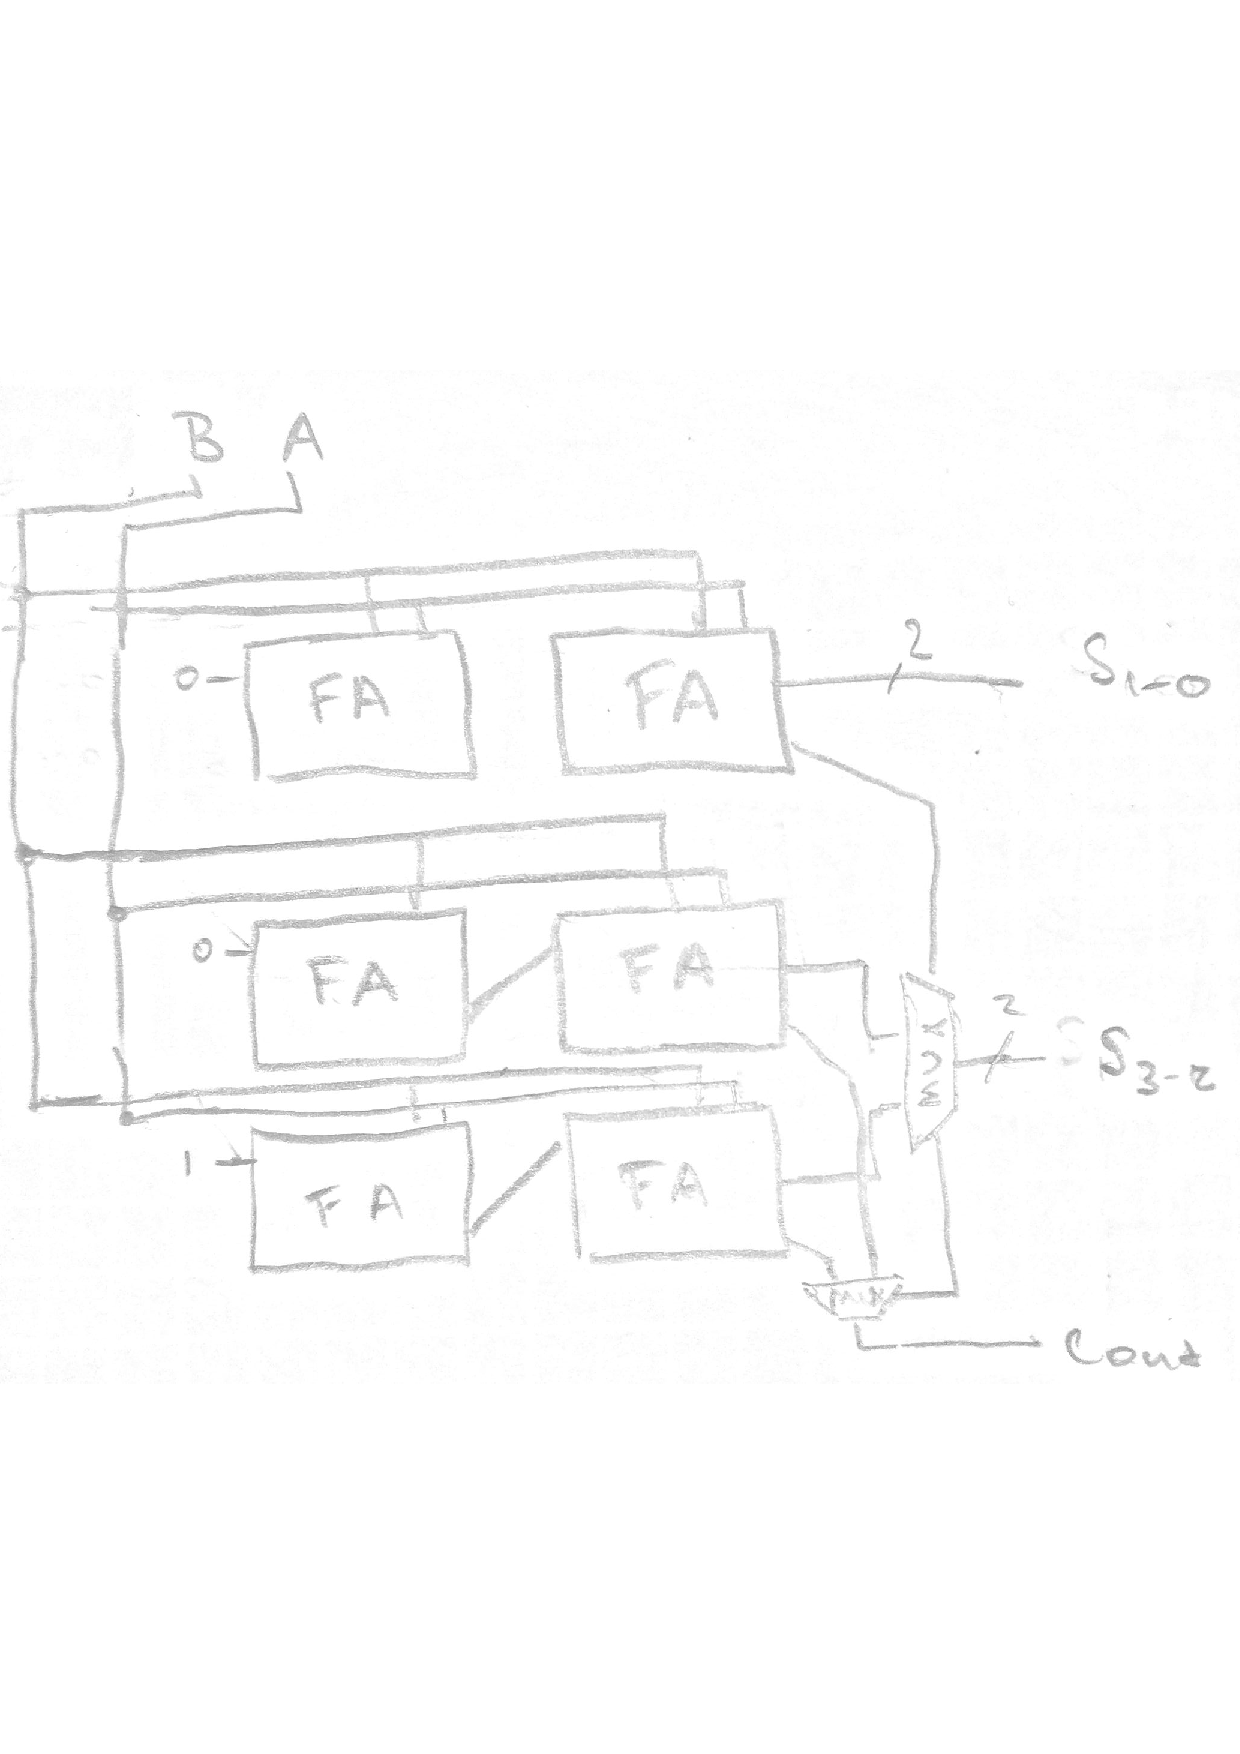
\includegraphics[width=7cm]{images/4b-CSA.pdf}
  \caption{An implementation of a 4 bit carry-select adder. Only block diagram is shown.}
  \label{fig:4csa}
\end{figure}

\subsection{Multipliers}

\section{Quiz}

\end{document}
